\documentclass[conference]{IEEEtran}
\IEEEoverridecommandlockouts
% The preceding line is only needed to identify funding in the first footnote. If that is unneeded, please comment it out.
\usepackage{cite}
\usepackage{amsmath,amssymb,amsfonts}
\usepackage{algorithmic}
\usepackage{graphicx}
\usepackage{textcomp}
\usepackage{xcolor}
\def\BibTeX{{\rm B\kern-.05em{\sc i\kern-.025em b}\kern-.08em
    T\kern-.1667em\lower.7ex\hbox{E}\kern-.125emX}}
\begin{document}

\title{The Research on IoT Botnet
\\
{\rightline{\large-- Use Mirai Botnet as an Example}}
}

\author{\IEEEauthorblockN{Fang Lin}
\IEEEauthorblockA{\textit{Freie Universit\"at Berlin} \\
IoT \& Security Seminar Report
}
}

\maketitle

% Abstract and key words
\begin{abstract}
The Internet of Things (IoT) is becoming an indispensable part of our daily lives, playing an increasingly important role in health, the environment, the family, the military and so on. The Internet of Things has grown tremendously in recent years. However, IoT devices still suffer from basic security vulnerabilities. Hackers use their computing and communication advantages to perform different types of attacks, IoT botnet is one of them. Mirai Botnet is the most typical type of Botnets. This article uses Mirai Bot as the main body of analysis. Firstly, the basics of IoT botnets will be introduces, some IoT vulnerabilities and famous IoT incidents will also be described. After this, I will go further to understand IoT botnets more by analysing the timeline of events, structure and propagation form of Mirai Botnet. By using some statistics, the behaviour and the spread of Mirai will be explained. Also this article will analyse  how to detect and prevent botnets, hoping to gain a deeper understanding of IoT botnets and how to prevent them. And the end, some discussions and conclusions will be written about the lessons learned from above already mentioned parts.
\end{abstract}

\begin{IEEEkeywords}
IoT, Botnet, Mirai Botnet, DDoS, Deep Learning
\end{IEEEkeywords}

% First Part, introduction
\section{\textbf{Introduction}}
The introduction part mainly introduces the background and significance of the research, some basic concepts, and the structure of this article.

\subsection{\textbf{Research Background}}
The IoT botnet is an important reason that makes IoT devices unable to operate normally and leads to network security issues such as the leakage of private information. IoT botnets mainly interfere with the operation of IoT devices by attacking DDoS. Looking back at the history of the IoT botnets invading the IoT devices, a series of network security incidents have occurred in the economic, smart city and so one. As a classic botnet, Mirai botnet is worthy of our in-depth research on botnets to explore the reasons for these things.
\subsection{\textbf{Research Significance}}
On the one hand, through the analysis and research of the Mirai botnet, I can have a deeper understanding of the botnet and also have a better understanding of the security issues of IoT devices. On the other hand, by understanding how to prevent the infringement of botnets, I can also improve my awareness of prevention when using IoT devices, that is, to be able to use IoT devices more sensibly, not to blindly believe and use without them security protection. they, so that the private information can be better protected.
\subsection{\textbf{Basic Concenpts}}
\begin{itemize}
\item \textbf{IoT}\\
he Internet of things (IoT) describes the network of physical objects—a.k.a. "things"—that are embedded with sensors, software, and other technologies for the purpose of connecting and exchanging data with other devices and systems over the Internet.\cite{b16}
\item \textbf{Botnet}\\
A botnet is a
network of infected machines or bots, also called zombies,
that has a command-and-control infrastructure
and is used for various malicious activities such as distributed
denial-of-service (DDoS) attacks.\cite{b10}
\item  \textbf{Mirai Botnet}\\
  The Mirai botnet, composed primarily of embedded
and IoT devices, took the Internet by storm in late 2016
when it overwhelmed several high-profile targets with
massive distributed denial-of-service (DDoS) attacks.\cite{b1}
\item  \textbf{DDoS}\\
In a distributed denial-of-service attack (DDoS attack), the incoming traffic flooding the victim originates from many different sources. This effectively makes it impossible to stop the attack simply by blocking a single source.\cite{b14}
\item  \textbf{Deep Learning}\\
Deep learning (also known as deep structured learning) is part of a broader family of machine learning methods based on artificial neural networks with representation learning. Learning can be supervised, semi-supervised or unsupervised.\cite{b15}
\end{itemize}
\subsection{\textbf{Structure}}
\begin{figure}[htbp]
\centerline{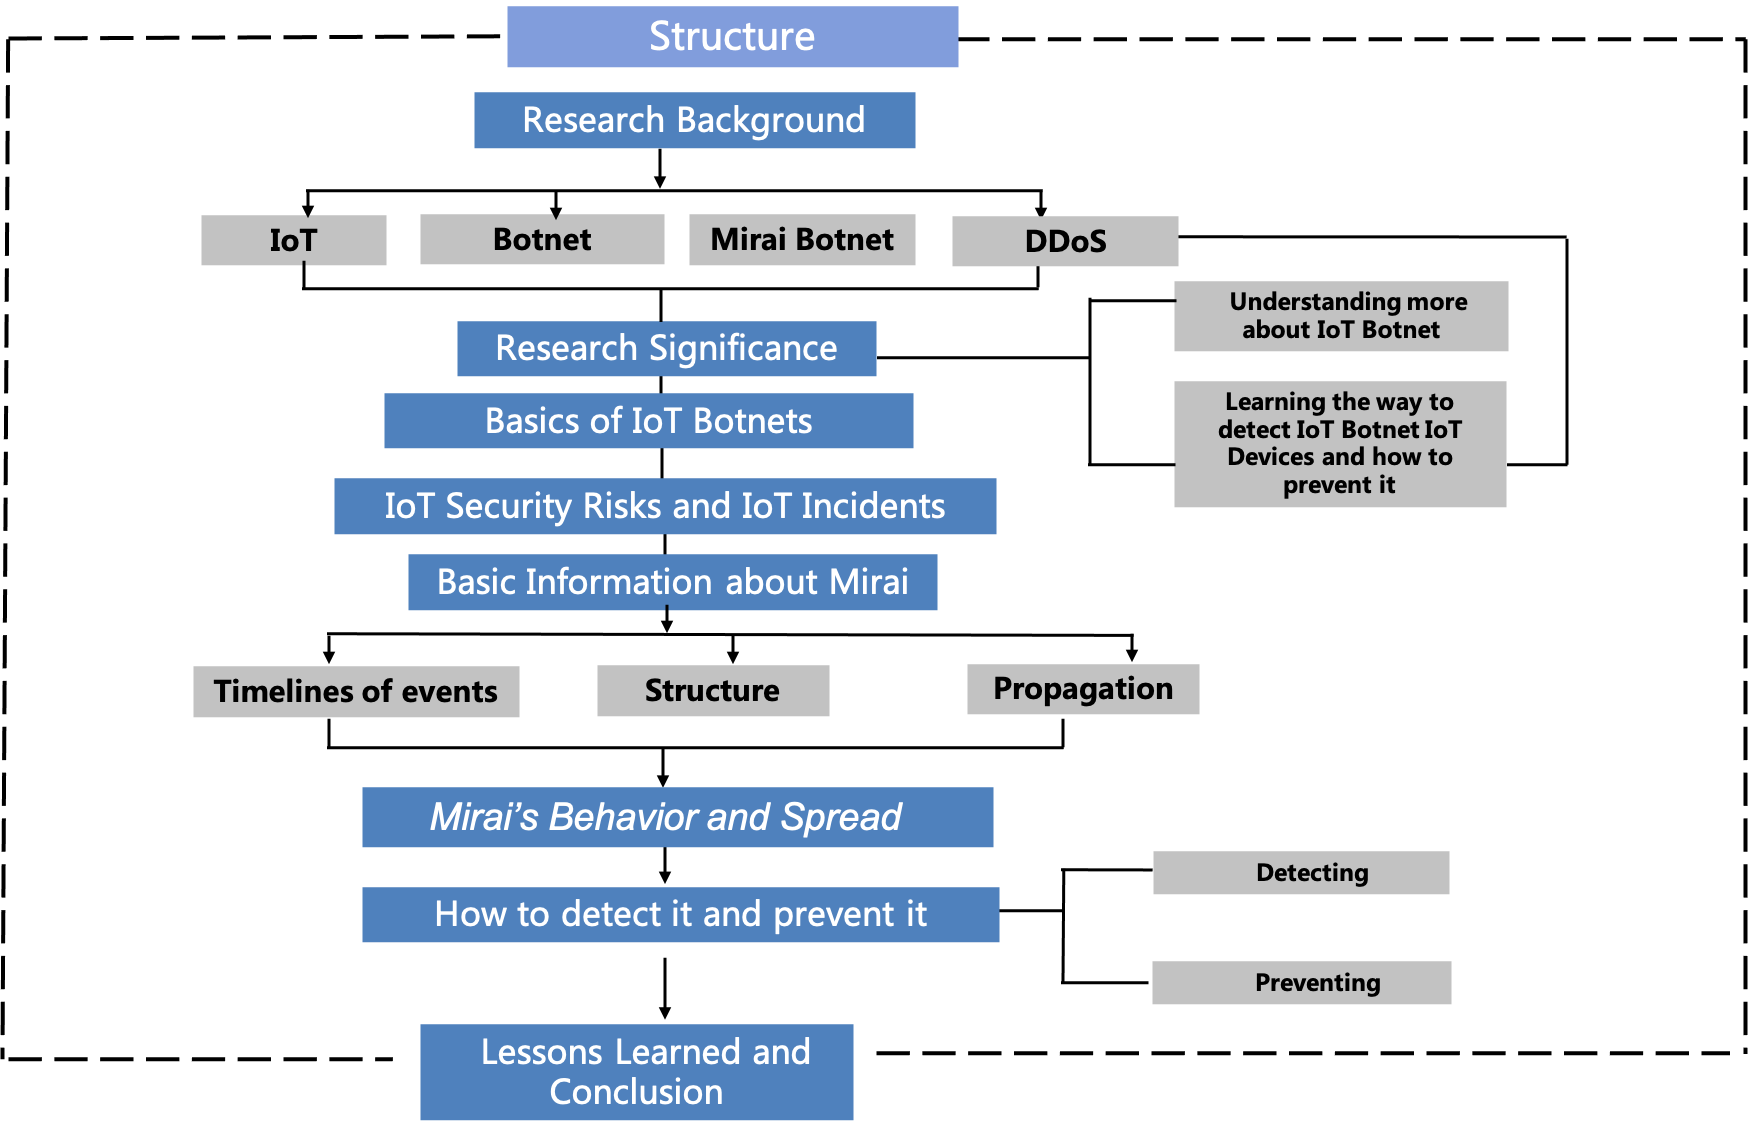
\includegraphics[scale=0.242]{structure.png}}
\caption{Structure of this article}
\label{fig}
\end{figure}

%The second part, introduces Basics of IoT Botnets
%


\section{\textbf{Basics of IoT Botnets }}
In this section, the basics of IoT botnets will be introduced. The IoT Security Risks and some famous IoT incidents will also be introduced here to understand more about IoT Bonets and why some incidents happened.
\subsection{\textbf{IoT Botnet Structure}}
\begin{figure}[htbp]
\flushleft{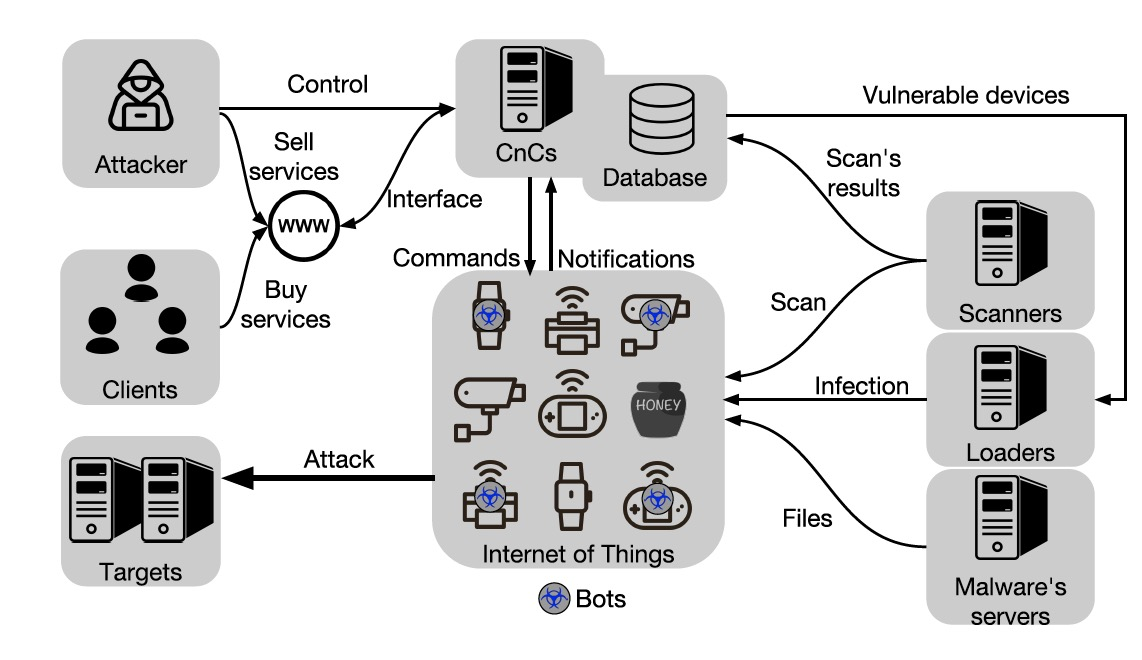
\includegraphics[scale=0.23]{overview.png}}
\caption{Overview of an IoT Botnet\cite{b3}}
\label{fig}
\end{figure}

\begin{itemize}
\item {The left part includes attackers, clients, and targets which are easy to understand. }
\begin{itemize}
\item {Attackers}\\
Attackers are those who try to attack the IoT devices to gain profits.

\item {Clients}\\
Clients are the groups who bought IoT devices and use them as a part of normal life, in the context they are also the victims.
\item {Targets}\\
Targets are the IoT devices which suffered from the attacks from the attackers and then the information of the clients may be exposed.
\end{itemize}
\item {The center  part includes three domains, which are CnCs, Database and Bots, these should be explained more detailed in the following.}
\begin{itemize}
\item {CnCs }\\
Command and control servers (C\&C) are the operators’
interface to the botnet. C\&Cs receive commands
from operators and maintain connections with infected
devices to broadcast commands.\cite{b3}}
\item {Database}\\
Database (potentially distributed) stores information collected
by the botnet, e.g., active bots and scan results.\cite{b3}}
\item {Bots }\\
Bots are infected devices that are part of the botnet.
Bots report their state to C\&Cs and execute the received
commands.\cite{b3}}
\end{itemize}

\item {In the right part there are scanners, loaders and malware's servers.}
\begin{itemize}
\item {Scanners}\\
Scanners probe devices to find telnet and SSH servers to
attempt login and identify vulnerable devices.\cite{b3}}

\item {Loaders}\\
Loaders login to vulnerable devices to download and run
the botnet malware, creating a new bot.\cite{b3}}

\item {Malware's servers}\\
Malware servers host resources used by the botnet such
as shell scripts and executable binaries.\cite{b3}}
\end{itemize}

\item{How will IoT devices be infected?}

\begin{itemize}
\item{ The scanner first identifies vulnerable devices and reports to the central database.}
\item{The loader then connects to the vulnerable device to download and run the malware. During the infection process, the loader accesses the server to download and run the malware binary file on the vulnerable device. }
\item{Once infected, the bot will connect to the C\&C of the botnet and wait for commands. To prevent subsequent infection attempts from other botnets, the IoT botnet disables the telnet and SSH services of the infected device. }
\item{Finally, operators may sell botnet services (for example, denial of service attacks), which are usually accessible through the client’s web interface }

\end{itemize}
\end{itemize}

\subsection{\textbf{Different Botnets}}

In this subsection  some botnets will be shortly introduced.

\begin{itemize}
\item{
\textbf{The first IoT botnet written in the
Lua programming language was reported
by MalwareMustDie in late August
2016.} Most of its army is composed
of cable modems with ARM CPUs
and using Linux. This malware incorporates
sophisticated features such
as an encrypted C&C communication
channel and customized iptables rules
to protect infected devices.\cite{b8}}

\item{
\textbf{The Hajime botnet, discovered in
October 2016 by Rapidity Networks,
uses a method of infection similar to
that of Mirai.\cite{b6}} However, rather than having a centralized architecture, Hijame
relies on fully distributed communications
and makes use of the
BitTorrent DHT (distributed hash tag)
protocol for peer discovery and the
uTorrent Transport Protocol for data
exchange. Every message is RC4 encrypted
and signed using public and
private keys. So far, Hajime hasn’t evidenced
malicious behavior; in fact,
it actually closes potential sources
of vulnerabilities in IoT devices that
Mirai- like botnets exploit, causing
some researchers to speculate that it
was created by a whitehat.But its
true purpose remains a mystery.}

\item{
\textbf{A BusyBox-based IoT botnet like
Mirai, BrickerBot was unearthed by
Radware researchers in April 2017.}
By leveraging SSH service default credentials,
misconfigurations, or known
vulnerabilities, this malware attempts
a permanent denial-of-service (PDoS)
attack against IoT devices using various
methods that include defacing
a device’s firmware, erasing all files
from its memory, and reconfiguring
network parameters.}

\item{
\textbf{
Linux/IRCTelnet is a new IRC botnet ELF malware aimed
at IoT devices with IPv6 capabilities. } IRCTelnet combining
the concept of Tsunami for IRC protocol, BASHLITE
for the infection techniques (telnet brute force access and
code injection) and using theMirai botnet’s IoT credential
list. The base source code of LightAidra/Aidra is used to
build the new botnet malware. The botnet is using UDP,
TCP flood along with other series of attack methods in
both IPv4 and IPv6 protocol. The new malware features
the extra IP spoof option in both IPv4 or IPv6.\cite{b2}}


\item{
\textbf{
Mirai is one of the most predominant DDoS IoT botnet in
recent times. Mirai means "the future" in Japanese. }Mirai
botnet is definitely the next step in IoT DDoS botnet malwares,
however not as sophisticated as Remaiten but most
effective. At its peak, Mirai infected 4000 IoT devices
per hour and currently it is estimated to have little more
than half a million infected active IoT devices. Mirai
botnet is famous for being used in the record breaking
1.1Tbps DDoS attack with 148000 IoT devices. Mirai
targets mostly CCTV cameras, DVRs, and home routers.
The source code for Mirai has been published by its
alleged author Paras Jha using his online pseudonym
"Anna-senpai" on the English-language hacking community
Hackforums as open-source . Since the release of
the Mirai source code, the number of IoT infected devices
has increased from 213000 to 483000 in just two weeks.
Based on the IP addresses one can identify that the Mirai
infected IoT devices are distributed in over 164 countries
with highest densities in Vietnam, Brazil, US, China and
Mexico. The strength of the DDoS attack
ranges from 200 Gbps to 1.2 Tbps. Mirai generates floods
of GRE IP, GRE ETH, SYN and ACK, STOMP, DNS,
UDP, or HTTP traffic against a target during a DDoS
attack. More recently, Mirai has been
found to be enhanced to infect Windows devices, helping
hackers hijack even more devices. This enhanced Mirai
malware could also identify and compromise database
services like MySQL and Microsoft SQL running on
different ports to create new admin "phpminds" with the
password "phpgodwith" allowing the hackers to steal the
database. The awareness of IoT botnets in recent times
attributes to Mirai and the volume of traffic generated
during its DDoS attacks.\cite{b2}}


\end{itemize}



\section{\textbf{IoT Security Risks and IoT incidents }}
In this section, the basics of IoT botnets will be introduced. The IoT Security Risks and some famous IoT incidents will also be introduced here to understand more about IoT Bonets and why some incidents happened.

\subsection{\textbf{IoT Security Risks}}
This chapter introduces some basick security risks of IoT so that we know why some attacks are easy to be taken.

\begin{itemize}
\item IoT systems have no clearly defined boundaries and are constantly changing due to the mobility of devices and users.
\item The IoT system is highly heterogeneous in terms of communication media and protocols, platforms and devices.
\item An IoT device can be an autonomous entity that controls other IoT devices.
\item An IoT system may include "things" that are not designed to connect to the Internet.
\item The IoT system or part of it may not be physically protected and/or controlled by different parties.
\item Unlike smartphone applications that require permission to install and interact with many users, due to the large number of devices, it may not be possible to make fine-grained permission requests in the IoT system.
\end{itemize}

In tabel I \cite{b10} lists the most common IoT vulnerabilities identified by the Open Web Application Security Project 
\begin{table}[htbp]
\caption{Common Internet of Things vulnerabilities.\cite{b10}}
\begin{center}
\begin{tabular}{p{80pt}p{150pt}}
 \hline
\textbf{Vulnerability} & \textbf{Examples} \\ 
 \hline
Insecure web/mobile/cloud interface & Inability to change default usernames and passwords; weak passwords;  lack of
robust password recovery mechanisms; exposed credentials; lack of account lockout;
susceptibility to cross-site scripting, cross-site request forgery, and/or SQL injection \\ 
 \hline
 Insufficient authentication/
authorization & Privilege escalation; lack of granular access control
Insecure\\
 \hline
 Insecure network services & Vulnerability to denial-of-service, buffer overflow, and fuzzing attacks; network ports
or services unnecessarily exposed to the Internet\\
 \hline
 Lack of transport encryption/integrity
verification & Transmission of unencrypted data and credentials\\
 \hline
 Privacy concerns & Collection of unnecessary user data; exposed personal data; insufficient controls on
who has access to user data; sensitive data not de-identified or anonymized; lack of data
retention limits\\
 \hline
 Insufficient security configurability & Lack of granular permissions model; inability to separate administrators from users;
weak password policies; no security logging; lack of data encryption options; no user
notification of security events\\
 \hline
 Insecure software/firmware &Lack of secure update mechanism; update files not encrypted; update files not verified
before upload; insecure update server; hardcoded credentials\\
 \hline
 Poor physical security & Device easy to disassemble; access to software via USB ports; removable storage media\\
  \hline
\end{tabular}
\label{tab1}
\end{center}
\end{table}

\subsection{\textbf{Some Incidents of IoT caused by Botnets }}
In this subsection some famous incidents of IoT caused by Botnets will be introduced, so that we can know which real things had happened by the attacking of IoT botnets.

\begin{itemize}
\item{ \textbf{KrebsOnSecurity.com}: On the evening of September 30, 2016, the blog of security researcher Brain Krebs experienced a 623Gbps DDoS attack from a large number of infected IoT devices \cite{b17}. This particular DDoS attack
was considered to be a retaliation action from a group of hackers due to Krebs’ series of articles on the take down of the Israeli DDoS-as-a-Service provider called vDOS, which coincided with the arrests of two 18 years old men named
in those articles as the founders of the service\cite{b18}. Krebs is a free customer of Akamai, a leading CDN operator that hosts his blog site and provides protection from DDoS attacks. As DDoS mitigation measures began to cause problems for Akamai's paying customers, after resisting the three-day attack, Akamai terminated its free contract with Krebs. The DDoS attack is so aggressive that the Akamai platform cannot handle the resources needed to mitigate the attack because it is almost twice the size of the second largest attack they have seen before.\\

 Mirai and BASHLITE attack infected these IoT devices.The attack traffic was mostly of GRE traffic and junk web traffic such as SYN, GET and POST floods from legitimate connections between attacking host and target.}

\item{\textbf{OVH}: OVH is a French cloud computing and hosting company that provides virtual private servers (VPS), dedicated servers and other network services. On September 22, 2016, OVH founder and CTO Octave Klaba posted the news and screenshots on his Twitter account, explaining that the OVH server is undergoing a series of DDoS attacks, many of which exceed 100 Gbps, a record The most serious single attack OVH reached 799 Gbps \cite{b19}. Later on September 23, 2016, Klaba once again posted on his Twitter account that OVH had experienced a record-breaking DDoS attack, generating at least 1.1 Tbps to 1.5 Tbps of traffic from the 145607 camera/DVR. The traffic sent by networked devices is between 1-30 Mbps. The attack is suspected to come from IoT devices infected with Mirai and BASHLITE malware. The traffic sent by it is mainly TCP/Ack, TCP/Ack+PSH and TCP/SYN \cite{b19}. The OVH attack did not give any reason, but it was the largest DDoS attack ever launched. The hacker with the pseudonym "Anna-senpai" released the Mirai botnet malware source code, claiming to have lived in France during the OVH attack, and evaded law enforcement by participating in the DDoS attack on KrebsOnSecurity.com.}

\item{\textbf{Dyn}: Dyn is an Internet performance management company that provides a wide range of products to monitor, control and optimize online infrastructure. Dyn is also one of the world's leading managed DNS providers. On October 21, 2016, Dyn suffered a DDoS attack on its hosted DNS server from 100,000 Internet-enabled IoT devices (such as printers, IP cameras, residential gateways, and baby monitors), which generated masks through port 53 TCP and UDP traffic. The IoT devices used in the attack were found to be mainly infected by Mirai botnet malware. According to some experts, the attack range reached 1.2 Tbps, but it has not yet been confirmed by Dyn. The attack was analyzed as a complex and complicated attack. In addition to the flooding of the masked TCP and UDP traffic, it also compounded the recursive DNS retry traffic, thereby further amplifying the impact of the attack. In other words, after the attack, the Dyn DNS server experienced 10-20 times the typical legitimate traffic from millions of IP addresses, because the recursive DNS server generated multiple DNS requests when the user retryed to visit the website. The DDoS attack itself was launched at two different time intervals. The first attack started from 11:10 to 13:20 UTC, and then from 15:50 UTC to 17:00 UTC. The first attack began at 11:10 UTC on the Dyn managed DNS platform in Asia Pacific, South America, Eastern Europe, and the Western United States, triggering Dyn’s response to initiate its incident response protocol. Dyn observed that the attack suddenly changed the target to their point of presence (POP) in the eastern United States. Dyn's engineering and network operations team began to deploy additional mitigation mechanisms, such as traffic shaping, rebalancing incoming traffic by adjusting anycast strategy, internal traffic filtering, and the deployment of cleaning services. The attack subsided at 13:20 UTC time, either because of Dyn's mitigation measures or the attacker's intention, so it is not clear. The second wave of attacks on the hosted DNS platform started again at 15:50 UTC time, coming from more IoT devices distributed around the world, but the mitigation mechanism that has been set up due to the first wave of attacks can be extended to the second attack, Dyn 17:00 UTC can be restored significantly. Residual effects from other sources were observed before 20:30 UTC time. Dyn reports that in the hours and days after the two waves of DDoS attacks, many smaller TCP attacks were observed.\\

Dyn provides hosted DNS services to some well-known websites (such as Airbnb, Amazon.com). Reddit, Spotify, and many other products that are partially or completely unavailable to users in Europe and North America.The impact of the outage due to DDoS attack on Dyn is illustrated in
the figure 3. According to Datanyze, a leading technology graphics provider that analyzes hosted DNS, Dyn is the most popular hosted DNS provider, providing services to 137 of the 1,000 top Alexa websites in 2015, but after DDoS attacks, Dyn was the most popular hosted DNS provider. They now only provide services to 90 of the 1,000 top Alexa sites, and have lost many customers to their main competitors Cloudflare DNS and Amazon Route 53, they market their services as hosted cloud DNS services.


\begin{figure}[htbp]
%\flushright
\flushleft{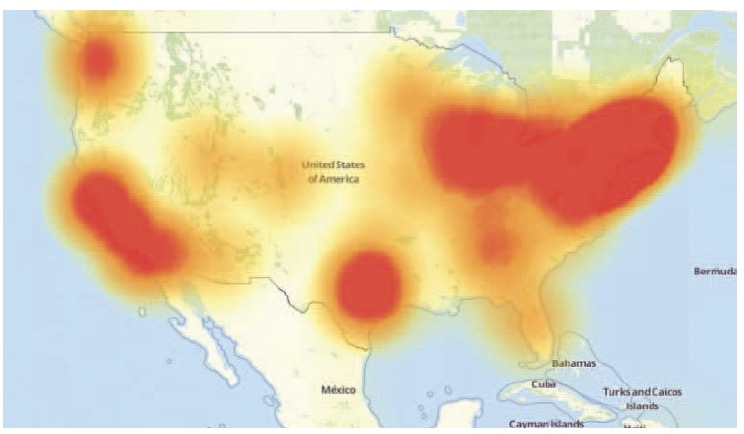
\includegraphics[scale=0.34]{depiction.jpg}}
\caption{Depiction of the outage caused in US by Dyn DDoS attack \cite{b2}}
\label{fig}
\end{figure}
}

\item{\textbf{Deutsche Telekom}: Deutsche Telekom is a German telecommunications company with strong influence in Europe and the United States. They are one of the most popular Internet service providers in Germany. Deutsche Telekom provides their DSL users with a home router with a built-in DSL modem, manufactured by a different company under the brand name "Speedport". On Sunday, November 27, 2016, a large number of Deutsche Telekom customers reported connection problems. These problems can be traced back to specific models of "Speedport" home routers, namely Speedport W 921V, Speedport W 723V Typ B, Speedport W 921 Fiber manufactured by Taiwanese manufacturer Arcadyan. It was discovered that the root cause of the problem was the new Mirai malware variant, which tried to actively scan and infect vulnerable devices in order to expand the number of infected devices in its botnet. The security researcher "kenzo2007" reported the vulnerabilities that these new Mirai malware variants intend to exploit on his blog dated November 7, 2016. Interestingly, Arcadyan, the Taiwanese manufacturer of vulnerable "Speedport" home routers for Deutsche Telekom, does not appear to be connected to Zyxel, the manufacturer of vulnerable Eir modems. The new Mirai malware variant exploits three different vulnerabilities.
\begin{itemize}
\item{Most ISP leave the port 7547 open on ISP supplied home
router / modem for remote management of CPE using
TR069 (CPE WAN Management Protocol). Though, this
is not a huge flaw, it is not recommended as anyone can
access CPE (router/modem) using the port 7547. The
authentication method used by TR069 either requires
no passwords or use weak HTTP digest authentication
method over unencrypted path or using certificate authentication,
which is in most cases not implemented
properly by the manufacturers. This issue was first
pointed out by security researcher Luka Perkov in his
talk "ISP Black Box" at 28C3 and more recently by
Shahar Tal in his talk " I Hunt TR-069 Admins: Pwning
ISPs Like a Boss" at DEFCON 22. A simple search
on Shodan (www.shodan.io) shows approximately 41
million devices have their port 7547 open.\cite{b2}

}
\item{
TR064 ( LAN-Side DSL CPE Configuration) Server was
running behind the port 7547 meant for TR069. TR064
strictly meant for local configuration of CPE but not
for remote management. This flaw allows anyone on
Internet to access CPE (Router/Modems) and perform
important device (CPE) configurations.\cite{b2}}
\item{
The crucial flaw in these specific models of CPE is
that "SetNTPServer" command of TR064 can be used
to execute arbitrary commands (command injection vulnerability).\cite{b2}}
\end{itemize}


\begin{figure}[htbp]
%\flushright
\flushright{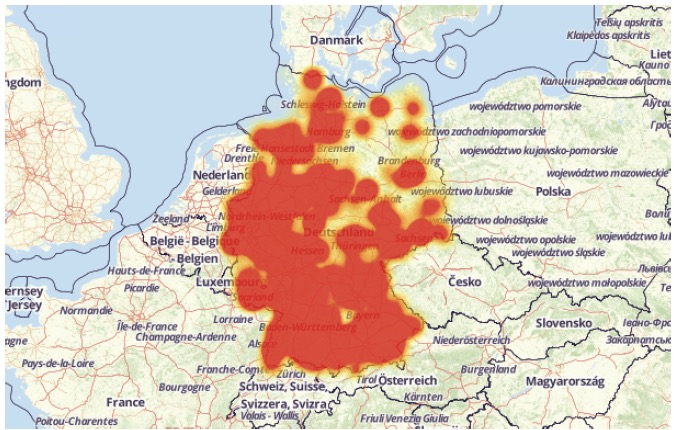
\includegraphics[scale=0.34]{positionslots.jpg}}
\caption{Depiction of the outage caused in Germany by Mirai attack on
Deutsche Telekom Customers \cite{b2}}
\label{fig}
\end{figure}

In \cite{b20} Comsecuris, a security company conducted some tests on one of the "Speedport" modems and found that it was not vulnerable, but they did observe that the modem became slow or not working properly even under moderate loads. So it is possible even though-although the new Mirai malware variant did not succeed, it caused the modem to crash. Mira IoT malware resides in the temporary memory (RAM) of the IoT device, so a simple power reset can remove the malware from the infected IoT device. However, many IoT botnet herders continue to scan the Internet, looking for vulnerable Internet-enabled IoT devices. According to the non-profit security agency SANS, the new Mirai variant constantly scans the Internet for new vulnerable devices and can find any newly connected router/modem within 10 minutes. A test conducted by security researcher Darren Martyn showed that the modems used by ISP TalkTalk, D-Link DSL 3780 modems, MitraStar, Digicom, and Aztech modems all have vulnerabilities. He said he has now found 48 different vulnerable devices in use. Deutsche Telekom reported that the incident affected 900,000 home routers, accounting for one in 20 Deutsche Telekom customers. Similar incidents have been reported by the UK ISP’s TalkTalk and the UK Post Office’s Internet broadband service, affecting more than 100,000 customers. Deutsche Telekom and other UK ISPs can fix security issues in vulnerable devices by providing firmware updates. Figure 4 illustrates the impact of the German outage due to the attack on the vulnerable "Speedport" home router by the new Mirai variant.}


\item{
\textbf{Liberia}: In early November, the @MiraiAttacks Twitter account observed an attack on Liberia's telecommunications infrastructure by the Mirai IoT botnet. This led to speculation that the Internet in Liberia was shut down by Mirai \cite{b2}1. A security researcher reported from an anonymous source that the 500 Gbps attack targeted Liberia’s submarine Internet cable, which further intensified speculation that the Mirai botnet might disrupt Liberia’s Internet access. This is consistent with the network connection problems observed by Liberian users. The general manager of the Liberia Cable Alliance reported that the Africa-Coast to Europe (ACE) submarine cable monitoring system and local servers located at the Liberian Internet Exchange Point (LIXP) did not experience downtime during the reporting period. However, Kpetermeni Siakor, who manages the LIXP infrastructure, informed that Lonestar Cell MTN, one of the four major telecommunications companies, faced a 500 Gbps DDoS attack in a short period of time, but it has been successfully mitigated.

}


\item{
\textbf{CCTV vs Small Business Websites}
A DDoS attack exploited thousands of websites like small jewelry shop websites. This attack lasted
for days and was from more than 25,000 compromised CCTV devices. 5% of the IPs observed in
this attack were IPv6.
}

\item{
\textbf{Lappeenranta}
In Lappeenranta, two housing blocks experienced disruption of heating distribution, which was due
to DDoS attack by the Mirai botnet. The system rebooted the central control to mitigate
the attack but got caught in an infinite restart loop. For more than a week, the heating system was
offline due to this infinite restart loop.
}


\item{\textbf{Russian Banks}
At least 5 Russian banks experienced a DDoS attack. Using this attack, 24,000 compromised IoT
devices were utilized which were distributed around 30 countries .
}


\item{\textbf{US Elections}
DDoS attacks were observed on the campaign website of Donald Trump and Hillary Clinton .
On 6th November 2016, the DDoS attack lasted for 24 hours on TCN, which was used by-election
campaigns . This attack started by sending a small flood of junk traffic but increased progressively
until all the connections got saturated.}

\item{\textbf{WikiLeaks}
A DDoS attack, which was nearly for 24 hours, made the email publication servers of Wikileaks to
be offline. This DDoS attack was in response to ”DNSLeak2”.}

\item{\textbf{Random DoS}
In Random denial of service (RDoS), Hackers sent ransom letters to organizations to inform them
they were exploited. Many cyber criminals utilized DDoS as a Service to send out some warning
shots and are reported to earn $100,000.}

\end{itemize}



% The third part, concentrate on Mirai Botnet
\section{\textbf{Basics of  Mirai Botnet}}
We have already introduce some basic concepts about IoT botnets and also some IoT incidents. We will find, many incidents are concerned with Mirai, why is Mirai so typical and caused so many incidents?  In this section, I will go further about the IoT Botnets by using Mirai Botnet as a specific example. I will mainly write the information of Mirai Botnet, including the timeline of events, the structure and the way of propagation.


%Timeline of events
\subsection{\textbf{The Timeline of Mirai Botnet }}

We already introduced some IoT incidents above, many are concerned with Mirai Botnets, so I will quickly explain the timeline of Mirai Botnet to not only make a small conclusion about the incidents mentioned above but also draw a clear line what Mirai Botnet has attacked.
\begin{figure}[htbp]
%\flushright
\flushright{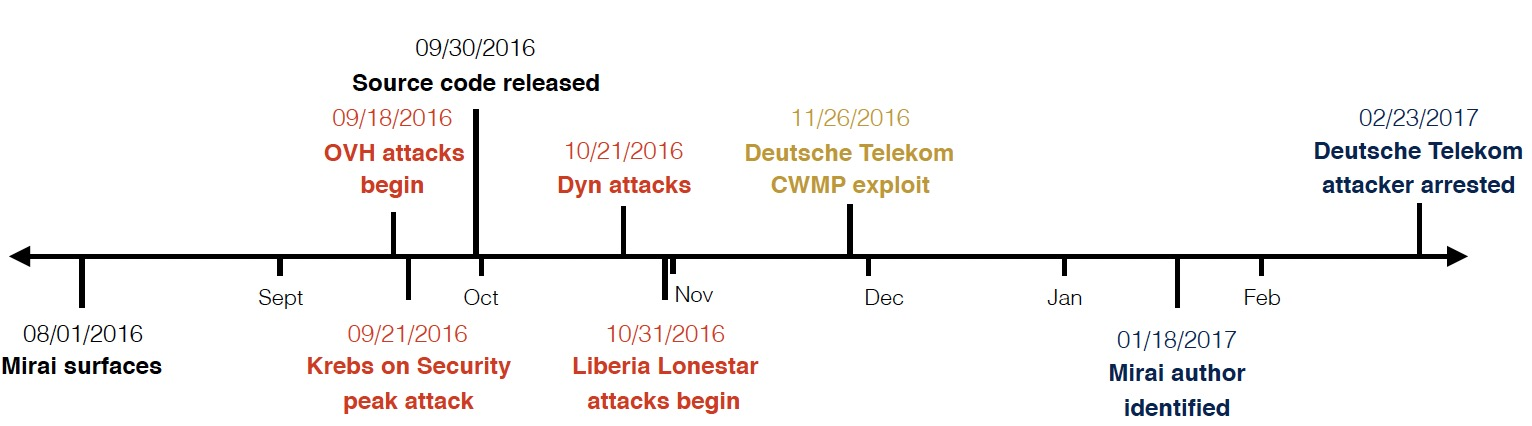
\includegraphics[scale=0.18]{timeline.png}}
\caption{Timeline of events: Major attacks (red), exploits (yellow), and events (black) related to the Mirai botnet.\cite{b1}}
\label{fig}
\end{figure}
From Figure 5\cite{b1}, we can see that on August 1, 2016, Mirai’s surfaces were released. Mirai’s first attack was on September 18, 2016, which was OVH attacks. On the 21st, it attacked DNS provider Dyn. During the two attacks, the source code was released on the Internet. At the end of November, it exploited the vulnerability of Deutsche Telekom CWMP. On January 18, 2017, the author of Mirai was confirmed and arrested at the end of February of the same year.

\subsection{\textbf{The Structure and Propagation of Mirai Botnet}}
This chapter introduces the structure and propagation of Mirai Botnet mainly by figure 6\cite{b1}, which basically follows the structure of an Iot Botnet, but will be more specific and orientational just about Mirai Botnet.

\begin{figure}[htbp]
\flushleft{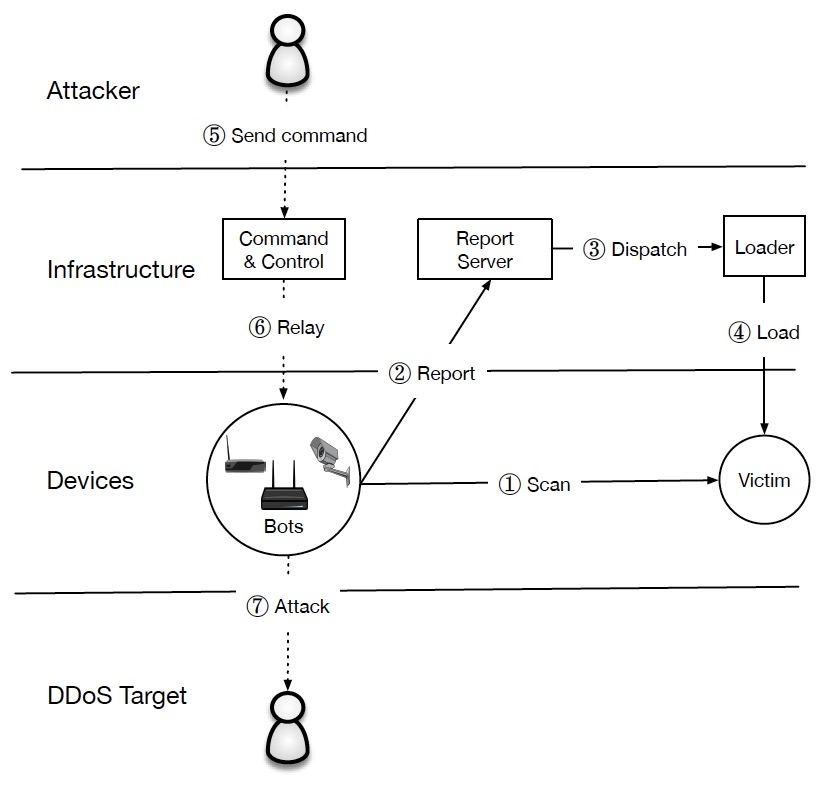
\includegraphics[scale=0.3]{mirai.png}}
\caption{\textbf{Mirai Operation}—Mirai bots scan the IPv4 address
space for devices that run telnet or SSH, and attempt to log in using
a hardcoded dictionary of IoT credentials. Once successful,
the bot sends the victim IP address and associated credentials to
a report server, which asynchronously triggers a loader to infect
the device. Infected hosts scan for additional victims and accept
DDoS commands from a command and control (C2) server.\cite{b1}}
\label{fig}
\end{figure}

\paragraph{\textbf{The Structure  of Mirai Botnet}}\\

Compare to figure 2,  the components of the structure of  Mirai Botnet are almost the same, except there is a report server of mirai botnet structure.
\textbf{Report Server} is a server which Bots will report the victim IP address to it.
In the figure 6\cite{b1}, four layers are designed to describe the mirai botnet structure.

\begin{itemize}
\item{ \textbf{Attacker}}\\
The same as in figure 2, it's the hackers who want to attack the IoT devices.
\item{\textbf{Infrastructure}}\\
In Infrastructure Layer, there are three components, C\&C, Roport Server and Loader.
\item{\textbf{Devices}}\\
The Devices layer is made of bots and victim, the victim here is the victim IoT device.
\item{\textbf{DDoS Targer}}\\
Easy to understand, it's the clients of an IoT devices, which their devices are attacked by Mirai Botnet.

\end{itemize}
\paragraph{\textbf{The Propagation of Mirai Botnet}}\\
As we can see in figure 6, there are 7 phases about the propagation of Mirai Botnet.



\begin{itemize}
\item{ \textbf{Phase 1}}\\
Mirai spread by first entering
a rapid scanning phase 1 where it asynchronously and
“statelessly” sent TCP SYN probes to pseudorandom IPv4
addresses, excluding those in a hard-coded IP blacklist, on
Telnet TCP ports 23 and 2323 (hereafter denoted TCP/23
and TCP/2323). If Mirai identifies a potential victim, it entered
into a brute-force login phase in which it attempted
to establish a Telnet connection using 10 username and
password pairs selected randomly from a pre-configured
list of 62 credentials.\cite{b1}
\item{ \textbf{Phase 2}}\\
At the first successful login, Mirai
sent the victim IP and associated credentials to a hardcoded
report server.
\item{ \textbf{Phase 3}\\
A separate loader program asynchronously infected
these vulnerable devices by logging in, determining
the underlying system environment.
\item{ \textbf{Phase 4}}\\
And at the end  this separate loader program infected the devices by downloading
and executing architecture-specific malware.

\item{ \textbf{Phase 5}}\\
The attackers will send the command to C\&C services.
\item{ \textbf{Phase 6}}\\
 The C\&C services relay the instruction from the attacker to certain bots.

\item{ \textbf{Phase 7}}\\
At the end, the bots will attack the DDoS Target.
\\

\item{ After a successful infection, Mirai attempted to conceal
its presence by deleting the downloaded binary and obfuscating
its process name in a pseudorandom alphanumeric
string. As a consequence, Mirai infections did not
persist across system reboots. In order to fortify itself,
the malware additionally killed other processes bound
to TCP/22 or TCP/23, as well as processes associated
with competing infections. At this point, the bot listened for attack commands from the command and control
server (C2) while simultaneously scanning for new
victims.\cite{b1}}
\end{itemize}




%The forth part, introduces how Mirai attacks IoT devices
\section{\textbf{ Watching Mirai's Behavior and Tracking Mirai’s Spread}}

In Chapter II I write the basic structure about Mirai Botnet and  I describe the propagation of the Mairi Botnet, it's actually the basic route how Mairi attacks IoT devices.
 In this Chapter I will go further about Mirai Botnet by summarising the analysis from article \cite{b1} in two aspects,  one is by using the network vantage
points: a large, passive network telescope, Internet-wide
scanning, active Telnet honeypots, logs of C2 attack
commands, passive DNS traffic, and logs from DDoS
attack targets to get the information about how Mirai Botnet behavior, another aspect is by tracking Mirai's Spread to know further how it works, and may contribute the our next chapter.
\subsection{\textbf{Mirai's Behavior}}

\paragraph{\textbf{Network Telescope}}\\
Mirai’s indiscriminate, rapid scanning strategy lends itself
to tracking the botnet’s propagation to new hosts. The authors\cite{b1}}
monitored all network requests to a network telescope
composed of 4.7 million IP address operated by Merit
Network over a seven month period from July 18, 2016
to February 28, 2017.

   On average, the network telescope
received 1.1 million packets from 269,000 IP addresses
per minute during this period. To distinguish Mirai traffic
from background radiation and other scanning activity,
we uniquely fingerprinted Mirai probes based on
an artifact of Mirai’s stateless scanning whereby every
probe has a TCP sequence number—normally a random
32-bit integer—equal to the destination IP address. The
likelihood of this occurring incidentally is 1=232, and we
would expect to see roughly 86 packets demonstrating
this pattern in our entire dataset. In stark contrast, we
observed 116.2 billion Mirai probes from 55.4 million IP
addresses. Prior to the emergence of Mirai, we observed
only three IPs that perform scans with this fingerprint.
Two of the IP addresses generated five packets; two on
TCP/80 and three on TCP/1002. The third IP address belongs
to Team Cymru, who conducts regular TCP/443
scans.
\paragraph{\textbf{Active Scanning}}\\
In order to determine the
manufacturer and model of devices infected with Mirai,
the authors \cite{b1} leveraged Censys, which actively scans the IPv4
space and aggregates application layer data about hosts on
the Internet.

A number of challenges make accurate device labeling
difficult. First, Mirai immediately disables common outward
facing services (e.g., HTTP) upon infection, which
prevents infected devices from being scanned. Second,
Censys scans often take more than 24 hours to complete,
during which devices may churn to new IP addresses. Finally,
Censys executes scans for different protocols on
different days, making it difficult to increase label specificity
by combining banners from multiple services. 

A conclusion is that devices with open
services that are not closed by Mirai (e.g., HTTPS and
FTP) can appear repeatedly in Censys banner scans during
our measurement window (due to churn) and thus lead to
over counting when compared across protocols. 
\paragraph{\textbf{Telnet Honeypots}}
In order to track the evolution of Mirai’s capabilities, the authors \cite{b1}  collected
binaries installed on a set of Telnet honeypots that masqueraded
as vulnerable IoT devices. At the end they extracted
the set of logins and passwords, IP blacklists, and C2 domains
from these binaries, identifying 67 C2 domains and
48 distinct username/password dictionaries (containing a
total 371 unique passwords).
\paragraph{\textbf{Passive \& Active DNS}}
Following the public release of Mirai’s source code, competing
Mirai botnet variants came into operation.  the authors \cite{b1}
disambiguated ownership and estimate the relative size
of each Mirai strain by exploring passive and active DNS
data for the 67 C2 domains that we found by reverse engineering
Mirai binaries. We also leveraged our DNS data
to map the IP addresses present in attack commands to
victim domain names. In total,  33 unique DNS
clusters of Mirai Botnet are identified.

\paragraph{\textbf{Attack Commands}}
To track the DDoS attack commands issued by Mirai
operators, Akamai ran a “milker” from September 27,
2016–February 28, 2017 that connected to the C2 servers found in the binaries uploaded to their honeypots. 

The authors \cite{b1}note that a naive analysis of attack
commands overestimates the volume of attacks and targets:
individual C2 servers often repeat the same attack
command in rapid succession, and multiple distinct C2
servers frequently issued the same command. 
\paragraph{\textbf{DDoS Attack Traces}}

For Google Shield, The authors \cite{b1} shared a list of IP addresses
observed by our network telescope and in turn
received aggregate statistics on what fraction matched
any of 158.8K IP addresses involved in a 1-minute Mirai
HTTP-flood attack on September 25, 2016. Finally, Dyn
provided them with a set of 107.5K IP addresses associated
with a Mirai attack on October 21, 2016.

\subsection{\textbf{Tracking Mirai's Spread}}

\paragraph{\textbf{Bootstrapping}}
Mirai’s comparatively modest initial
growth may be due to the low bandwidth and computational
resources of infected devices, a consequence of the
low-accuracy, brute-force login using a small number of
credentials, or simply attributable to a bottleneck in loader
infrastructure.
\paragraph{\textbf{Steady State Size}}
The authors \cite{b1} observed multiple phases in Mirai’s life: an initial
steady state of 200,000–300,000 infections in September
2016; a peak of 600,000 infections at the end of November
2016; and a collapse to roughly 100,000 infections at
the end of our observation window in late February 2017
(Figure 3). Even though hosts were initially compromised
via a simple dictionary attack, Mirai was able to infect
hundreds of thousands of devices. This is similar in scale
to historical botnets such as the prolific Srizbi spam botnet
(400,000 bots ), which was responsible for more
than half of all global botnet spam , and the Carna
botnet (420,000 bots), the first botnet of IoT devices
compromised using default credentials.
\paragraph{\textbf{Global Distribution}}
Where Mirai infections were geographically
concentrated?

\begin{figure}[htbp]
\flushleft{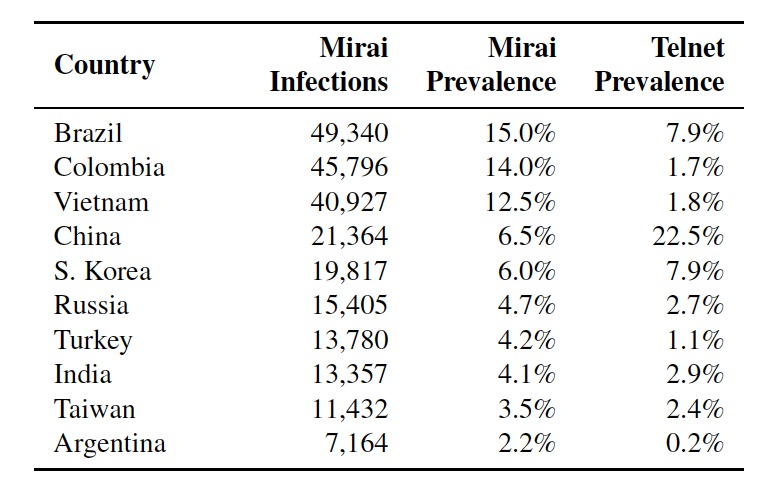
\includegraphics[scale=0.33]{geo.png}}
\caption{Geographic Distributiont\cite{b1}}
\label{fig}
\end{figure}

In figure 7 we can see, most Mirai infections originate from
Located in Brazil (15.0\%), Colombia (14.0\%) and
Vietnam (12.5\%)

\paragraph{\textbf{Device Composition}}

While cursory evidence suggested that Mirai targets IoT
devices—Mirai’s dictionary of default usernames and
passwords included routers, DVRs, and cameras.

After the gathering and analysing of the authors \cite{b1}, the devices they identified were primarily
network-attached storage appliances, home routers, cameras,
DVRs, printers, and TV receivers made by dozens
of different manufacturers.

The manufacturers responsible
for the most infected devices we could identify are:
Dahua, Huawei, ZTE, Cisco, ZyXEL, and MikroTik.

The data indicates that some of the world’s top manufacturers
of consumer electronics lacked sufficient security
practices to mitigate threats like Mirai, and these
manufacturers will play a key part in ameliorating vulnerability.
Unfortunately, as discussed in the previous
section, the menagerie of devices spanned both countries
and legal jurisdictions, exacerbating the challenge of coordinating
technical fixes and promulgating new policy to
safeguard consumers in the future.
\paragraph{\textbf{Device Bandwidth}}
Mirai was primarily powered by devices with limited
computational capacity and/or located in regions with low
bandwidth.

%Fourth Section, how to detect it and prevent it.
\section{\textbf{How to detect and prevent IoT Botnets}}



\subsection{\textbf{Detecting}}
Different approaches used to detect IoT botnet at different steps of botnet life cycle. The approaches
used to detect IoT botnet are discussed in the following subsections.

\paragraph{\textbf{Anomaly-based}}

This approach detects IoT botnet by recognizing malicious behavior in the network; this approach
requires storing previous profile for the normal behavior for the network. Summerville et al, developed
an ultralight packet anomaly-based method to detect abnormal payload in the packet, using efficient matching
technique for bit pattern requires only ADD operation followed by incremental counter, and implemented as
a look up table for fast and flexible packet evaluation. Sagirlar et al,  proposed Auto Bot catcher, which
utilizes Block chain concept to detect decentralized P2P Botnets. The design of AutoBotCatcher is driven
by the concept that bots in the same botnets usually communicate with each other and form a community,
so it will detect the community by analyzing the network traffic between IoT devices and then detect the
botnet. AutoBotCatcher consists of two main actors: agents and block generator. The agent is responsible
for monitoring the network traffic between IoT devices, and sending the collected information as a block chain
transaction to a big trusted entity in the network (block generator), which will model mutual contact information
of IoT device and create mutual contact graph, and then use Louvain method  to detect community based
on the graph. \cite{b4}
\paragraph{\textbf{Signature-based}}

This approach detects the IoT botnet based on the signature of the botnet stored in the database of the
system. P. Ioulianou et al proposed a solution that depends on Intrusion Detection System (IDS), which
is a security technology used to monitor networks for any malicious activity or policy violation. They place
these IDS modules in a hybrid mode. The detection and firewall module called Router IDS and the monitoring
lightweight module called Detector IDS. These modules are distributed in the network close to IoT devices,
and this does not require any software modification on sensors or devices. Detector IDS logs network traffic
and sends it to the Router IDS that will detect malicious node behavior if it resembles to a known attack.
Khoshhalpour et al,  proposed a host-based approach called BotRevealer to detect IoT botnet in the early
infection step, using botnet life cycle as a general signature for detection. They analyze the running process and
network activities on the host based on statistical features of packet sequence and compare it with the behavior
pattern of botnet traffic.\cite{b4}


\paragraph{\textbf{Specification-based}}
This approach is similar to anomaly-based approach but it takes into account system specifications.
Carli et al, proposed an automatic interference technique for the specifications of malware network
protocol using samples of malware communication and malware binary. Since each malware has its own
custom binary format and each C$&$C protocol has its own malware family, this will provide a fingerprint for the
malware structure and intent. They proposed a type system field of the message that describes all field types
in the message, and then use type interference algorithm to interfere message structure. However, most C$&$C
network traffic is encrypted so they apply dynamic traffic analysis to extract C$&$C system keys. Prokofiev et al
 proposed a detection technique for IoT botnets during the propagation stage where infected devices starts
to exploit other devices in the network using brute-force attack using telnet and/or ssh protocols. They build
a logistic regression model based on the Request Parameters and Specification such as: (Destination Port, even
number of requests and alphanumeric) to estimate IoT bot. initiates the probability that the connection initiated
to a device. They build the model using the data collected from 100 IoT Botnets. \cite{b4}
\paragraph{\textbf{Hybrid-based}}

This approach combines two approaches together, anomaly-based and signature-based techniques or
anomaly-based and specification-based techniques, to detects the IoT botnet with high detection and low false
positive rate. Sedjelmaci et al proposed a low energy consumption anomaly and signature based, to detect
attacks effectively using the proposed Game Theory to model the security strategy as a game formula between
the attacks and the IDS agent in the IoT device, and use Nash equilibrium to determine the equilibrium state that
will allow the IDS agent to activate the anomaly detection technique only when the attack signature is expected
to happen, this will reduce the power consumption in IoT device due to anomaly detection techniques and
increase the detection accuracy. In the other hand, Bostani et al proposed anomaly-based and specificationbased
intrusion detection models to detect attacks in IoT. The specification-based detection agent will be
located on routers nodes; it will analyze the host node behaviour and send the results to the root node where
the anomaly-based detection agent is located. This agent based on the Map reduce architecture will employ
optimum path algorithm using the data sent by routers nodes to project clustering model and detect malicious
behaviour using voting mechanism. \cite{b4}
\paragraph{\textbf{A novel graph-based approach}}

 In  paper \cite{b5}, they propose a lightweight method for detecting IoT
botnet, which based on extracting high-level features from function–call graphs, called PSI-Graph, for each executable file.
This feature shows the effectiveness when dealing with the multi-architecture problem while avoiding the complexity of
control flow graph analysis that is used by most of the existing methods. The experimental results show that the proposed
method achieves an accuracy of 98.7\%, with the dataset of 11,200 ELF files consisting of 7199 IoT botnet samples and 4001
benign samples. Additionally, a comparative study with other existing methods\cite{b5}

\paragraph{\textbf{Botnet detection
systems using DNS queries}}
\begin{itemize}
\item{\textbf{String similarity detection\cite{b13}}}
\begin{itemize}
\item{Homoglyph or name spoofing attacks are used to obfuscate domain names, and their existing methods rely on string matching and Levenshtein or edit distance functions, which are computationally heavy and produce high false positive results.The method based on edit distance would classify a legitimate domain as a spoof and a spoofed domain as real.}


\item{Consequently, multiple studies proposed name spoofing detection techniques based on visual comparisons. Some developers developed custom edit distance functions, which are dependent on the visual similarity of characters. Replacement of character by a visually similar character could result in a smaller edit distance than a visually different character. The techniques depend on manually derived similarity measures between the characters, and they did not include a sizeable Unicode set. 
}
\item{
A metric-learning technique based on a siamese convolutional neural network (S-CNN) model for detecting domain and process homoglyph attacks is proposed. The proposed model was trained on the strings rendered as images for detecting the visual similarity of the strings. }
\end{itemize}


\item{\textbf{DGA detection based deep
learning\cite{b13}}}
\begin{itemize}
\item{Woodbridge
et al. presented a feature-less real-time DGA classifier,
which uses a long short-term memory (LSTM) network. The
performance of the classifier outperformed the random forest
(RF) model using manually-crafted features.}
\item{ In \cite{b13}, the
authors introduced a method by discussing various issues related to synthetic data,
explicit labeling and proposed a deep learning approach for
DGA detection to overcome the issues. They trained LSTM,
convolutional neural network (CNN), and RF with a large
volume of real-time data and presented a detailed comparative
analysis. }
\item{Yu et al. compared the performance of
a recurrent neural network (RNN) and CNN deep learning
models, which perform a character-based text classification
for detecting DGAs. The outputs of the models are almost the
same in terms of accuracy and false positive rates.}
\item{Lison et al. proposed an RNN deep learning model
for detecting malicious domain names generated by DGAs.
The model was trained on a large data set, which contains
samples with a total of 61 malware families.}
\end{itemize}

\end{itemize}

\paragraph{\textbf{one class support vector
machine and Grey Wolf optimization for IoT botnet detection\cite{b12}}}

In this paper, a new unsupervised evolutionary IoT botnet detection method is proposed. The main contribution of the proposed method is to detect IoT botnet attacks launched form compromised IoT
devices by exploiting the efficiency of a recent swarm intelligence algorithm called Grey Wolf Optimization algorithm
(GWO) to optimize the hyperparameters of the OCSVM and at the same time to find the features that best describe the IoT
botnet problem. To prove the efficiency of the proposed method, its performance is evaluated using typical anomaly detection
evaluation measures over a new version of a real benchmark dataset. The experimental results show that the proposed method
outperforms all other algorithms in terms of true positive rate, false positive rate, and G-mean for all IoT device types. Also,
it achieves the lowest detection time, while significantly reducing the number of selected features\cite{b12}.

\subsection{\textbf{Preventing}}
This Chapter is about some basic techniques that we can use to avoid the attacks from Botnet and also some IoT security strategies which can prevent IoT devices from suffering the attacks from Botnets.
\paragraph{\textbf{Protection Techniques }}
Ensuring that IoT devices aren’t exploited
as zombies requires adopting a
few well-known security practices that
address the most common vulnerabilities. There are some basic pretection techniques which we can use to avoid the attacks.
\begin{itemize}
\item{ensuring that all default passwords
are changed to strong
passwords;}
\item{updating IoT devices with security
patches;}
\item{disabling Universal Plug and
Play (UPnP) on routers unless
absolutely necessary;}
\item{monitoring IP ports /TCP
and /TCP for attempts to gain
unauthorized control over IoT
devices using the network terminal
(Telnet)}
\item{monitoring for anomalous
tra c on port , as infected
devices often attempt to spread malware by using this port to
send results to the threat actor.}
\item{specific end-user actions such as only
acquiring IoT devices from companies
with a good security reputation and
understanding the devices’ communication
capabilities, as they’re at higher
risk of malware infection.}
\end{itemize}



\paragraph{\textbf{ Longer-Term IoT Security Strategy}}
Mirai is just the first of a new type of botnet that utilizes IoT devices and systems. Unfortunately, as history has shown, the deployment of defenses against a given security threat will soon emerge with new attack methods. Therefore, we will soon anticipate more complex attacks than Mirai, and even more devastating consequences. In particular, since many IoT systems and devices have driving capabilities and can change the physical environment, attacks on such systems and devices may cause major security risks and endanger human lives. Designing security technologies specific to the Internet of Things must be a research focus.\\


Defenses against conventional botnets can be broadly categorized into prevention, monitoring, and response.
\begin{itemize}
\item{Preventing bot infection is the most effective defense measure. This can be achieved through antivirus software and intrusion prevention systems, firewalls, content filtering and inspection technologies, and application whitelists. User awareness is also important, because malware is often spread due to user errors, such as clicking on email attachments.}
\item{However, despite the use of security technology, the machine can still be infected. Therefore, it is important to monitor network and device behavior for abnormal events or trends that may indicate threats. Network Behavior Analysis (NBA) programs-which can be installed and operated by administrators or provided by third-party services-continuously monitor data flows from routers and other sources, and flag traffic, bandwidth usage, protocol usage, and other indicators that deviate from established baselines.}
\item{Users can also take a more active role in threat detection by reporting typical machine infection signs such as longer start-up or shut-down times, frequent crashes, unexplained error messages, and unusually slow operation. More specific, see the following tips from \cite{b9}}
\begin{itemize}
\item{Always replace default manufacturer passwords immediately upon use. }
\item{Keep the firmware for devices current and up to date}
\item{For IP camera and similar systems that require remote access, invest in a VPN.}
\item{Disable unnecessary services (e.g., Telnet) and close ports that are not required for the IoT device.}

\end{itemize}
\item{If signs of a potential DDoS attack or infected machine are detected, prompt response is essential to minimize damage and prevent the spread of malware. Responses can range from simple operations (such as disconnecting a suspicious machine from the network) to tracking, analyzing, and shutting down the botnet. NBA tools can perform some mitigation measures—for example, they can use Border Gateway Protocol or similar routing mechanisms to redirect potentially malicious traffic to other hosts. However, advanced operations such as disabling botnets may require the participation of professional security companies or law enforcement agencies.
\item{Deploying these various defenses won’t be trivial given the large number of IoT devices and their inherent vulnerabilities. It’s thus essential to extend existing security mechanisms such as encryption, authentication, access control, network security, and application security to fit the IoT ecosystem. For example, techniques and tools are needed to analyze firmware for flaws such as authentication bypass back doors.}
\item{Devising methods for discovering, identifying, and monitoring IoT devices is also critical. For example, the adoption of stronger passwords and/or a whitelist of addresses from which it’s possible to log into IoT devices and to which IoT devices can send traffic would have prevented the exploitation of such devices by the Mirai botnet.}
\item{The security strategy must also include a thorough risk assessment. However, an important advantage to keep in mind is that many IoT devices today have specialized functions with very limited inputs, so their behavior is very predictable. This makes it easier to establish baseline operations in monitoring tools to detect anomalies that may indicate potential attacks or equipment damage. In order to maintain the scalability of this method, such monitoring activities can be performed through IoT routers or gateways.}
\end{itemize}


%Last Section, how to detect it and prevent it.
\section{\textbf{Lessoned Learned and Conclusion}}
\subsection{\textbf{Lessoned Learned }}
\begin{itemize}
\item{The security challenges facing IoT devices are much
more difficult to deal with. There are many ways an adversary
can access a smart appliance. An adversary can
directly get access to the device, or get access to the mobile
phone, tablet, or a thermostat that controls that device,
or with the ubiquity of digital home assistant devices
such as Amazon Alexa or Google Home, an adversary
can control smart appliances by getting access to
these devices. Any of these devices can be a breaching
point for an adversary. Hence, coherent security measures
are needed to protect almost all the devices within
a home network against an adversary.
Thus, in the IoT side, more research is required to study
the vulnerability of IoT devices and networks, and to protect
them against cyber attacks.\cite{b11}}
\item{The huge impact of Mirai, its variants, and other botnet-like DDoS attacks highlights the risks that IoT devices pose to the Internet. Currently, even naive methods can control such devices and create a large and extremely destructive army of zombie devices. The susceptibility and stability of the generated robot population are attractive factors for any attacker. There are five main reasons why IoT devices are particularly useful for creating botnets: \cite{b8}}
\begin{itemize}
\item{Poor maintenance. Most IoT devices belong to the set and forget umbrella-after initially setting them, users and network administrators will forget them unless they stop working properly.}
\item{A large amount of attack traffic. Contrary to popular belief, IoT devices are powerful enough and well located to generate DDoS attack traffic comparable to modern desktop systems.}
\item{Non-interactive or minimally interactive user interface. Since IoT devices often require minimal user intervention, infections are more likely to go unnoticed. Even if they are noticed, there is no easy way for users to solve them unless the device is replaced.}
\item{Continuous and unobtrusive operation. Unlike laptops and desktop computers that frequently switch on and off, many IoT devices (such as webcams and wireless routers) operate 24/7, and in many cases cannot be correctly identified as computing devices.}
\item{Weak protection. In the process of eager to penetrate the Internet of Things market, many equipment suppliers neglected security, and tended to user-friendliness and usability.}
\end{itemize}
\item{The Mirai botnet shows that even a simple dictionary attack can compromise hundreds of thousands of connected devices. Although a random default password is the first step, future attacks are likely to evolve into software vulnerabilities in IoT devices. In order to mitigate this threat before the threat begins, IoT security must evolve from the default open port to the default closed port, and adopt security hardening best practices. Devices should consider the default network configuration and restrict remote address access of these devices to the local network or specific providers. In addition to network security, IoT developers also need to apply ASLR, isolation boundaries, and principles of least privilege in their designs. From a compliance perspective, certification may help guide consumers to make safer choices and force manufacturers to produce safer products.}
\item{Automatic updates — which have become the norm in the desktop and mobile operating systems world — provide developers with a timely mechanism to fix bugs and vulnerabilities without burdening consumers with maintenance tasks or requiring recalls. Automatic updates require a modular software architecture to safely cover core modules with rollback capabilities in the event of a failure. They also need encryption primitives for resource-constrained devices and build PKI infrastructure to support trusted updates. In addition to these challenges, patching also requires the IoT community to actively self-monitor vulnerabilities, which is a potentially onerous responsibility given the diversity of devices.}
\item{IoT manufacturers can use a unified way to identify the network model and firmware version—for example, by encoding them into a part of the device's MAC address. Disclosing this information at Layer 2 will make it visible to local network operators (or users’ home routers), and they may one day take automated steps to disable remote access to known vulnerable hardware until it is updated. Achieving this goal in a uniform manner across the industry may require the adoption of standards.}
\item{Although most IoT systems are closed and tailored for specific applications, due to the number and diversity of devices, communication media, communication protocols, and software, such systems pose huge security challenges. Therefore, even testing IoT systems can be very difficult. In addition to scalability and interoperability issues, the IoT ecosystem also includes many different participants, each of which performs security-related functions-assigning identifiers to IoT devices, patching device software, and so on. Tracking information, such as device keys and who is responsible for which. In large-scale distributed systems with multiple security/management domains, the security aspects of devices are complex and critical.}
\item{After the research of many IoT articles, some aspects are still not that clear explained.The impacts of significant customization of the
botnet was not studied, and might be a topic for future research,although such customizations may be numerous and difficult to
predict.\cite{b7}}
\end{itemize}
\subsection{\textbf{Conclusion}}

This research is based on the Internet of Things botnet and has studied many aspects. Starting from the basic concepts, I first understand the basic structure and attack methods of IoT, and then introduce some classic IoT accidents. Many of these events are related to the Mirai botnet, which is one reason why I plan to focus on the Mirai botnet. By introducing the timeline of the Mirai botnet and its basic structure, comparing its spread with the Iot Botnet, and observing its behavior and spread through some data, we have a clearer concept of the Mirai botnet. Then, through a brief introduction of some methods of detecting IoT botnets, to understand what forms of detection are available, this section does not provide a more in-depth introduction, such as the development of a certain method. Then, I put forward some preventive measures and strategies, and finally discussed the lessons learned, mainly for some of the more important features and the work to be done in the future.

Through this extensive research and focus on understanding Mirai Botnet, I have a deeper understanding of IoT botnet. IoT devices have some vulnerabilities that are easy to be attacked. IoT botnet is not the only attack method. In the future, I may be interested in reading some articles on IoT device security to conduct more in-depth research on IoT security, and a more in-depth study of some technical aspects of detection methods which is not that comprehensive in this article, like machine learning, deep learning technics for the Botnet detection.

%\section*{References}


%\begin{thebibliography}{00}
%\bibitem{b1} G. Eason, B. Noble, and I. N. Sneddon, ``On certain integrals of Lipschitz-Hankel type involving products of Bessel functions,'' Phil. Trans. Roy. Soc. London, vol. A247, pp. 529--551, April 1955.
%\bibitem{b2} J. Clerk Maxwell, A Treatise on Electricity and Magnetism, 3rd ed., vol. 2. Oxford: Clarendon, 1892, pp.68--73.
%\bibitem{b3} I. S. Jacobs and C. P. Bean, ``Fine particles, thin films and exchange anisotropy,'' in Magnetism, vol. III, G. T. Rado and H. Suhl, Eds. New York: Academic, 1963, pp. 271--350.
%\bibitem{b4} K. Elissa, ``Title of paper if known,'' unpublished.
%\bibitem{b5} R. Nicole, ``Title of paper with only first word capitalized,'' J. Name Stand. Abbrev., in press.
%\bibitem{b6} Y. Yorozu, M. Hirano, K. Oka, and Y. Tagawa, ``Electron spectroscopy studies on magneto-optical media and plastic substrate interface,'' IEEE Transl. J. Magn. Japan, vol. 2, pp. 740--741, August 1987 [Digests 9th Annual Conf. Magnetics Japan, p. 301, 1982].
%\bibitem{b7} M. Young, The Technical Writer's Handbook. Mill Valley, CA: University Science, 1989.
%\end{thebibliography}
%\vspace{12pt}



\begin{thebibliography}{00}

\bibitem{b1}Manos Antonakakis, Georgia Institute of Technology; Tim April, Akamai; Michael Bailey, University of Illinois, Urbana-Champaign; Matt Bernhard, University of Michigan, Ann Arbor; Elie Bursztein, Google; Jaime Cochran, Cloudflare; Zakir Durumeric and J. Alex Halderman, University of Michigan, Ann Arbor; Luca Invernizzi, Google; Michalis Kallitsis, Merit Network, Inc.; Deepak Kumar, University of Illinois, Urbana-Champaign; Chaz Lever, Georgia Institute of Technology; Zane Ma and Joshua Mason, University of Illinois, Urbana-Champaign; Damian Menscher, Google; Chad Seaman, Akamai; Nick Sullivan, Cloudflare; Kurt Thomas, Google; Yi Zhou, University of Illinois, Urbana-Champaign.Understanding the Mirai Botnet. (2017)
\\Source: https://www.usenix.org/conference/usenixsecurity17/technical-sessions/presentation/antonakakis


\bibitem{b2} Kishore Angrishi. Turning Internet of Things(IoT) into Internet of Vulnerabilities (IoV) : IoT Botnets. (2017)
\\Source: https://arxiv.org/pdf/1702.03681.pdf

\bibitem{b3} Artur Marzano, David Alexander, O. Fonseca, E. Fazzion, C. Hoepers, Klaus Steding-Jessen, M. H. P. Chaves, Ítalo S. Cunha, D. Guedes, W. Meira .The Evolution of Bashlite and Mirai IoT Botnets. 2018 IEEE Symposium on Computers and Communications (ISCC) 
\\Source: https://honeytarg.cert.br/honeypots/docs/papers/honeypots-iscc18.pdf


\bibitem{b4}Basheer Al-Duwairi, Wafaa Al-Kahla, Mhd Ammar AlRefai, Yazid Abdelqader, Abdullah Rawash, Rana Fahmawi. SIEM-based detection and mitigation of IoT-botnet DDoS attacks. (2019) 
\\Source: https://www.researchgate.net/publication/340357755\_SIEM-based\_detection\_
and\_mitigation\_of\_IoT-botnet\_DDoS\_attacks


\bibitem{b5}Huy-Trung Nguyen, Quoc-Dung Ngo, Van-Hoang Le. A novel graph-based approach for IoT botnet detection. (2019) 
\\Source: https://link.springer.com/article/10.1007/s10207-019-00475-6


\bibitem{b6}Stephen Herwig, Katura Harvey, George Hughey, Richard Roberts, Dave Levin. Measurement and Analysis of Hajime, a Peer-to-peer IoT Botnet. (2019) 
\\Source:  https://www.ndss-symposium.org/wp-content/uploads/2019/02/ndss2019\_02B-3\_Herwig\_paper.pdf


\bibitem{b7}Xiaolu Zhang, Oren Upton, Nicole Lang Beebe, Kim-Kwang Raymond Choo. IoT Botnet Forensics: A Comprehensive Digital Forensic Case Study on Mirai Botnet Servers. (2020) 
\\Source:  https://www.sciencedirect.com/science/article/pii/S2666281720300214

\bibitem{b8} Constantinos Kolias, George Mason University, Georgios Kambourakis, University of the Aegean Angelos Stavrou, George Mason University Jeffrey Voas, IEEE Fellow. DDoS in the IoT: Mirai and Other Botnets. (2017) 
\\Source: https://ieeexplore.ieee.org/document/7971869

\bibitem{b9}Priscilla Moriuchi, Sanil Chohan. Mirai-Variant IoT Botnet Used to Target Financial Sector in January 2018. (2018)
\\Source:  https://go.recordedfuture.com/hubfs/reports/cta-2018-0405.pdf

\bibitem{b10}Elisa Bertino, Purdue University, Nayeem Islam, Qualcomm. Botnets and Internet of Things Security. (2017) 
\\Source: https://ieeexplore.ieee.org/document/7842850

\bibitem{b11}Saleh Soltan, Prateek Mittal, and H. Vincent Poor, Princeton University. BlackIoT: IoT Botnet of High Wattage Devices Can Disrupt the Power Grid. (2018) 
\\Source: https://www.usenix.org/conference/usenixsecurity18/presentation/soltan
\bibitem{b12}Amaal Al Shorman, Hossam Faris, Ibrahim Aljarah. Unsupervised intelligent system based on one class support vector machine and Grey Wolf optimization for IoT botnet detection. (2019) 
\\Source:  https://link.springer.com/article/10.1007/s12652-019-01387-y

\bibitem{b13}Vinayakumar R, Mamoun Alazab Senior Member, IEEE, Sriram S, Quoc-Viet Pham, Soman KP, Simran K. A Visualized Botnet Detection System based Deep Learning for the Internet of Things Networks of Smart Cities. (2020) 
\\Source: https://ieeexplore.ieee.org/document/8985278
\bibitem{b14}https://en.wikipedia.org/wiki/Denial-of-service\_attack
\bibitem{b15}https://en.wikipedia.org/wiki/Deep\_learning
\bibitem{b16}https://en.wikipedia.org/wiki/Internet\_of\_things
\bibitem{b17}B. Krebs. "KrebsOnSecurity hit with record
DDoS," in KrebsonSecurity. (2016). \\Source:
https://krebsonsecurity.com/2016/09/krebsonsecurity-hit-with-record-ddos/

\bibitem{b18}B. Krebs. "Alleged vDOS Proprietors Arrested
in Israel," in KrebsonSecurity. (2016). \\Source:
https://krebsonsecurity.com/2016/09/alleged-vdos-proprietors-arrested-in-israel/


\bibitem{b19}R. Millman. "OVH suffers 1.1Tbps DDoS attack,"
in News, SC Magazine UK. (2016) \\Source:
http://www.scmagazineuk.com/ovh-suffers-11tbps-ddos-attack/article/524826/ 

\bibitem{b20}Ralf. "Were 900K Deutsche Telekom Routers Compromised
by Mirai?". (2016). \\Source:https://comsecuris.com/blog/posts/were$\_$900k\_deutsche\_telekom
\_routers\_compromised\_by\_mirai/

\bibitem{21}B. Krebs. "Did the Mirai Botnet really take
Liberia Offline?," in KrebsonSecurity. 2016. \\Source:
https://krebsonsecurity.com/2016/11/did-the-mirai-botnet-really-take-liberia-offline/ 
\end{thebibliography}
\vspace{12pt}








\end{document}
